% Options for packages loaded elsewhere
\PassOptionsToPackage{unicode}{hyperref}
\PassOptionsToPackage{hyphens}{url}
\PassOptionsToPackage{dvipsnames,svgnames,x11names}{xcolor}
%
\documentclass[
  11pt,
  a4paper,
]{report}

\usepackage{amsmath,amssymb}
\usepackage{setspace}
\usepackage{iftex}
\ifPDFTeX
  \usepackage[T1]{fontenc}
  \usepackage[utf8]{inputenc}
  \usepackage{textcomp} % provide euro and other symbols
\else % if luatex or xetex
  \usepackage{unicode-math}
  \defaultfontfeatures{Scale=MatchLowercase}
  \defaultfontfeatures[\rmfamily]{Ligatures=TeX,Scale=1}
\fi
\usepackage{lmodern}
\ifPDFTeX\else  
    % xetex/luatex font selection
\fi
% Use upquote if available, for straight quotes in verbatim environments
\IfFileExists{upquote.sty}{\usepackage{upquote}}{}
\IfFileExists{microtype.sty}{% use microtype if available
  \usepackage[]{microtype}
  \UseMicrotypeSet[protrusion]{basicmath} % disable protrusion for tt fonts
}{}
\makeatletter
\@ifundefined{KOMAClassName}{% if non-KOMA class
  \IfFileExists{parskip.sty}{%
    \usepackage{parskip}
  }{% else
    \setlength{\parindent}{0pt}
    \setlength{\parskip}{6pt plus 2pt minus 1pt}}
}{% if KOMA class
  \KOMAoptions{parskip=half}}
\makeatother
\usepackage{xcolor}
\usepackage[top=2.5cm,bottom=2.5cm,left=2.5cm,right=2.5cm]{geometry}
\setlength{\emergencystretch}{3em} % prevent overfull lines
\setcounter{secnumdepth}{2}


\providecommand{\tightlist}{%
  \setlength{\itemsep}{0pt}\setlength{\parskip}{0pt}}\usepackage{longtable,booktabs,array}
\usepackage{calc} % for calculating minipage widths
% Correct order of tables after \paragraph or \subparagraph
\usepackage{etoolbox}
\makeatletter
\patchcmd\longtable{\par}{\if@noskipsec\mbox{}\fi\par}{}{}
\makeatother
% Allow footnotes in longtable head/foot
\IfFileExists{footnotehyper.sty}{\usepackage{footnotehyper}}{\usepackage{footnote}}
\makesavenoteenv{longtable}
\usepackage{graphicx}
\makeatletter
\newsavebox\pandoc@box
\newcommand*\pandocbounded[1]{% scales image to fit in text height/width
  \sbox\pandoc@box{#1}%
  \Gscale@div\@tempa{\textheight}{\dimexpr\ht\pandoc@box+\dp\pandoc@box\relax}%
  \Gscale@div\@tempb{\linewidth}{\wd\pandoc@box}%
  \ifdim\@tempb\p@<\@tempa\p@\let\@tempa\@tempb\fi% select the smaller of both
  \ifdim\@tempa\p@<\p@\scalebox{\@tempa}{\usebox\pandoc@box}%
  \else\usebox{\pandoc@box}%
  \fi%
}
% Set default figure placement to htbp
\def\fps@figure{htbp}
\makeatother
% definitions for citeproc citations
\NewDocumentCommand\citeproctext{}{}
\NewDocumentCommand\citeproc{mm}{%
  \begingroup\def\citeproctext{#2}\cite{#1}\endgroup}
\makeatletter
 % allow citations to break across lines
 \let\@cite@ofmt\@firstofone
 % avoid brackets around text for \cite:
 \def\@biblabel#1{}
 \def\@cite#1#2{{#1\if@tempswa , #2\fi}}
\makeatother
\newlength{\cslhangindent}
\setlength{\cslhangindent}{1.5em}
\newlength{\csllabelwidth}
\setlength{\csllabelwidth}{3em}
\newenvironment{CSLReferences}[2] % #1 hanging-indent, #2 entry-spacing
 {\begin{list}{}{%
  \setlength{\itemindent}{0pt}
  \setlength{\leftmargin}{0pt}
  \setlength{\parsep}{0pt}
  % turn on hanging indent if param 1 is 1
  \ifodd #1
   \setlength{\leftmargin}{\cslhangindent}
   \setlength{\itemindent}{-1\cslhangindent}
  \fi
  % set entry spacing
  \setlength{\itemsep}{#2\baselineskip}}}
 {\end{list}}
\usepackage{calc}
\newcommand{\CSLBlock}[1]{\hfill\break\parbox[t]{\linewidth}{\strut\ignorespaces#1\strut}}
\newcommand{\CSLLeftMargin}[1]{\parbox[t]{\csllabelwidth}{\strut#1\strut}}
\newcommand{\CSLRightInline}[1]{\parbox[t]{\linewidth - \csllabelwidth}{\strut#1\strut}}
\newcommand{\CSLIndent}[1]{\hspace{\cslhangindent}#1}

\usepackage{fvextra}
\DefineVerbatimEnvironment{Highlighting}{Verbatim}{
  commandchars=\\\{\},
  breaklines, breaknonspaceingroup, breakanywhere
}
\makeatletter
\@ifpackageloaded{bookmark}{}{\usepackage{bookmark}}
\makeatother
\makeatletter
\@ifpackageloaded{caption}{}{\usepackage{caption}}
\AtBeginDocument{%
\ifdefined\contentsname
  \renewcommand*\contentsname{Table of contents}
\else
  \newcommand\contentsname{Table of contents}
\fi
\ifdefined\listfigurename
  \renewcommand*\listfigurename{List of Figures}
\else
  \newcommand\listfigurename{List of Figures}
\fi
\ifdefined\listtablename
  \renewcommand*\listtablename{List of Tables}
\else
  \newcommand\listtablename{List of Tables}
\fi
\ifdefined\figurename
  \renewcommand*\figurename{Figure}
\else
  \newcommand\figurename{Figure}
\fi
\ifdefined\tablename
  \renewcommand*\tablename{Table}
\else
  \newcommand\tablename{Table}
\fi
}
\@ifpackageloaded{float}{}{\usepackage{float}}
\floatstyle{ruled}
\@ifundefined{c@chapter}{\newfloat{codelisting}{h}{lop}}{\newfloat{codelisting}{h}{lop}[chapter]}
\floatname{codelisting}{Listing}
\newcommand*\listoflistings{\listof{codelisting}{List of Listings}}
\makeatother
\makeatletter
\makeatother
\makeatletter
\@ifpackageloaded{caption}{}{\usepackage{caption}}
\@ifpackageloaded{subcaption}{}{\usepackage{subcaption}}
\makeatother

\usepackage{bookmark}

\IfFileExists{xurl.sty}{\usepackage{xurl}}{} % add URL line breaks if available
\urlstyle{same} % disable monospaced font for URLs
\hypersetup{
  pdftitle={Msc Bioinformatics thesis},
  pdfauthor={Valentin Goupille},
  colorlinks=true,
  linkcolor={blue},
  filecolor={Maroon},
  citecolor={Blue},
  urlcolor={Blue},
  pdfcreator={LaTeX via pandoc}}

%% CAPTIONS
\usepackage{caption}
\DeclareCaptionStyle{italic}[justification=centering]
 {labelfont={bf},textfont={it},labelsep=colon}
\captionsetup[figure]{style=italic,format=hang,singlelinecheck=true}
\captionsetup[table]{style=italic,format=hang,singlelinecheck=true}

%% FONT
\usepackage{bera}
\usepackage[charter]{mathdesign}
\usepackage[scale=0.9]{sourcecodepro}
\usepackage[lf,t]{FiraSans}
\usepackage{fontawesome}

%% HEADERS AND FOOTERS
\usepackage{fancyhdr}
\pagestyle{fancy}
\rfoot{\Large\sffamily\raisebox{-0.1cm}{\textbf{\thepage}}}
\makeatletter
\lhead{\textsf{\expandafter{\@title}}}
\makeatother
\rhead{}
\cfoot{}
\setlength{\headheight}{15pt}
\renewcommand{\headrulewidth}{0.4pt}
\renewcommand{\footrulewidth}{0.4pt}
\fancypagestyle{plain}{%
\fancyhf{} % clear all header and footer fields
\fancyfoot[C]{\sffamily\thepage} % except the center
\renewcommand{\headrulewidth}{0pt}
\renewcommand{\footrulewidth}{0pt}}

%% MATHS
\usepackage{bm,amsmath}
\allowdisplaybreaks

%% GRAPHICS
\makeatletter
\def\fps@figure{htbp}
\makeatother
\setcounter{topnumber}{2}
\setcounter{bottomnumber}{2}
\setcounter{totalnumber}{4}
\renewcommand{\topfraction}{0.85}
\renewcommand{\bottomfraction}{0.85}
\renewcommand{\textfraction}{0.15}
\renewcommand{\floatpagefraction}{0.8}
\graphicspath{{figures/}}

%% SECTION TITLES
\usepackage[compact,sf,bf]{titlesec}
\titleformat*{\section}{\Large\sf\bfseries}
\titleformat*{\subsection}{\large\sf\bfseries}
\titleformat*{\subsubsection}{\sf\bfseries}
\titlespacing{\section}{0pt}{*5}{*1}
\titlespacing{\subsection}{0pt}{*2}{*0.2}
\titlespacing{\subsubsection}{0pt}{*1}{*0.1}

%% TABLES
\usepackage{booktabs,tabu}

%% BIBLIOGRAPHY.

\makeatletter
\@ifpackageloaded{biblatex}{
\ExecuteBibliographyOptions{bibencoding=utf8,minnames=1,maxnames=3, maxbibnames=99,dashed=false,terseinits=true,giveninits=true,uniquename=false,uniquelist=false,doi=false, isbn=false,url=true,sortcites=false}
\DeclareFieldFormat{url}{\texttt{\url{#1}}}
\DeclareFieldFormat[article]{pages}{#1}
\DeclareFieldFormat[inproceedings]{pages}{\lowercase{pp.}#1}
\DeclareFieldFormat[incollection]{pages}{\lowercase{pp.}#1}
\DeclareFieldFormat[article]{volume}{\mkbibbold{#1}}
\DeclareFieldFormat[article]{number}{\mkbibparens{#1}}
\DeclareFieldFormat[article]{title}{\MakeCapital{#1}}
\DeclareFieldFormat[article]{url}{}
\DeclareFieldFormat[inproceedings]{title}{#1}
\DeclareFieldFormat{shorthandwidth}{#1}
\usepackage{xpatch}
\xpatchbibmacro{volume+number+eid}{\setunit*{\adddot}}{}{}{}
% Remove In: for an article.
\renewbibmacro{in:}{%
  \ifentrytype{article}{}{%
  \printtext{\bibstring{in}\intitlepunct}}}
\AtEveryBibitem{\clearfield{month}}
\AtEveryCitekey{\clearfield{month}}
\DeclareDelimFormat[cbx@textcite]{nameyeardelim}{\addspace}
\renewcommand*{\finalnamedelim}{\addspace\&\space}
}{}
\makeatother


\hypersetup{
     pdfcreator={Quarto -> pandoc -> LaTeX -> pdf}
}


%% PAGE BREAKING to avoid widows and orphans
\clubpenalty = 2000
\widowpenalty = 2000
\usepackage{microtype}
\def\maketitle{
\pagenumbering{roman}
{\sf\thispagestyle{empty}%
  \null\vskip-.4cm%
  % Logos at the top
  \begin{center}
    
\includegraphics[width=4cm]{logo_Univ_Rennes.png}\hspace{2cm}
    \includegraphics[width=4cm]{Logo_Université_Rennes_1.png}\hspace{2cm}
  \end{center}
  \vspace*{2cm}
  
  % Title and main information
  \begin{center}
    \fontsize{24}{28}\sf
    \textbf{Msc Bioinformatics thesis}\\[1cm]
    \textbf{Study of Division of Labor in Pseudomonas throught
single-cell RNA-seq}\\[1cm]
    \fontsize{18}{20}\sf
    Valentin Goupille\\[0.5cm]
    
    \fontsize{16}{18}\sf 
    Master 2 in Bioinformatics\\[0.5cm]
    
    \fontsize{14}{16}\sf
    Academic Year: 2024-2025\\[1cm]
    
    \fontsize{14}{16}\sf
    Internship conducted at Ecobio UMR 6553 CNRS-University of
Rennes\\[0.5cm]
  \end{center}
  % Logos at the bottom
  \begin{center}
    
\includegraphics[width=4cm]{logo-ecobio.png}
  \end{center}
  \begin{center}
    Ecobio UMR 6553 CNRS-University of Rennes\\[0.5cm]
    Campus de Beaulieu, 35042 Rennes Cedex, France\\[0.5cm]
  \end{center}
  \begin{center}
    \fontsize{14}{16}\sf
    \vspace{1cm}
    Under the supervision of:\\[0.3cm]
    \fontsize{14}{16}\sf
    Solène Mauger-Franklin, Postdoctoral Researcher\\[0.3cm]
    \fontsize{14}{16}\sf
    Philippe Vandenkoornhuyse, Professor\\[0.3cm]
  \end{center}
  
  \vfill
  
  % Submission date
  \begin{center}
    \fontsize{14}{16}\sf 
    Presented on 2025-07-01
  \end{center}
  
  \newpage\mbox{}\thispagestyle{empty}\newpage
}
}

% Title and date

\title{Msc Bioinformatics thesis}
\usepackage{etoolbox}
\makeatletter
\providecommand{\subtitle}[1]{% add subtitle to \maketitle
  \apptocmd{\@title}{\par {\large #1 \par}}{}{}
}
\makeatother
\subtitle{Study of Division of Labor in Pseudomonas throught single-cell
RNA-seq}
\date{}
\begin{document}
\maketitle

\renewcommand*\contentsname{Table of contents}
{
\hypersetup{linkcolor=}
\setcounter{tocdepth}{1}
\tableofcontents
}

\setstretch{1.5}
\bookmarksetup{startatroot}

\chapter*{Copyright notice}\label{copyright-notice}
\addcontentsline{toc}{chapter}{Copyright notice}

\markboth{Copyright notice}{Copyright notice}

Produced on 2 June 2025.

© Valentin Goupille (2025).

\bookmarksetup{startatroot}

\chapter*{Declaration}\label{declaration}
\addcontentsline{toc}{chapter}{Declaration}

\markboth{Declaration}{Declaration}

\subsection*{Statement of originality}\label{statement-of-originality}
\addcontentsline{toc}{subsection}{Statement of originality}

\begin{figure}[h]
    \raggedleft
    
\includegraphics[width=200px]{figures/logo_Univ_Rennes.png}
\end{figure}

I, the undersigned, \textbf{Valentin Goupille}, a student in the
\textbf{Master's program in Bioinformatics}, hereby declare that I am
fully aware that plagiarism of documents or parts of documents published
on any type of medium, including the internet, constitutes a violation
of copyright laws as well as an act of fraud.

As a result, I commit to citing all the sources I have used in the
writing of this document.

Date : \textbf{01/04/2025}

Signature :


\includegraphics[width=2.08333in,height=\textheight,keepaspectratio]{figures/signature.png}

\subsection*{Reproducibility statement}\label{reproducibility-statement}
\addcontentsline{toc}{subsection}{Reproducibility statement}

This thesis is written using Quarto. All materials (including the data
sets and source files) required to reproduce this document can be found
at the Github repository
\href{https://github.com/vgoupille/Internship_2025}{\texttt{github.com/vgoupille/Internship\_2025}}.

This work is licensed under a
\href{https://creativecommons.org/licenses/by-nc-nd/4.0/deed.en}{Attribution-NonCommercial-NoDerivatives
4.0 International License}.

\begin{figure}[h]
    \centering
    
\includegraphics[width=75px]{figures/CC_BY-NC-ND.png}
\end{figure}

\bookmarksetup{startatroot}

\chapter*{Abstract}\label{abstract}
\addcontentsline{toc}{chapter}{Abstract}

\markboth{Abstract}{Abstract}

\subsection*{Study of Pseudomonas brassicacearum gene expression
variation in environ-mental constraints, towards the validation of
Division Of
Labor.}\label{study-of-pseudomonas-brassicacearum-gene-expression-variation-in-environ-mental-constraints-towards-the-validation-of-division-of-labor.}
\addcontentsline{toc}{subsection}{Study of Pseudomonas brassicacearum
gene expression variation in environ-mental constraints, towards the
validation of Division Of Labor.}

Etiam quis tortor luctus, pellentesque ante a, finibus dolor. Phasellus
in nibh et magna pulvinar malesuada. Ut nisl ex, sagittis at
sollicitudin et, sollicitudin id nunc. In id porta urna. Proin porta
dolor dolor, vel dapibus nisi lacinia in. Pellentesque ante mauris,
ornare non euismod a, fermentum ut sapien. Proin sed vehicula enim.
Aliquam tortor odio, vestibulum vitae odio in, tempor molestie justo.
Praesent maximus lacus nec leo maximus blandit.

Maecenas turpis velit, ultricies non elementum vel, luctus nec nunc.
Nulla a diam interdum, faucibus sapien viverra, finibus metus. Donec non
tortor diam. In ut elit aliquet, bibendum sem et, aliquam tortor. Donec
congue, sem at rhoncus ultrices, nunc augue cursus erat, quis porttitor
mauris libero ut ex. Nullam quis leo urna. Donec faucibus ligula eget
pellentesque interdum. Lorem ipsum dolor sit amet, consectetur
adipiscing elit. Aenean rhoncus interdum erat ut ultricies. Aenean
tempus ex non elit suscipit, quis dignissim enim efficitur. Proin
laoreet enim massa, vitae laoreet nulla mollis quis.

\subsection*{Keywords :}\label{keywords}
\addcontentsline{toc}{subsection}{Keywords :}

Single-cell RNA-seq, Pseudomonas brassicacearum, Division Of Labor, (4-5
keywords) bacterial population, metabolism, specialization, root
colonization

\bookmarksetup{startatroot}

\chapter*{Acknowledgements}\label{acknowledgements}
\addcontentsline{toc}{chapter}{Acknowledgements}

\markboth{Acknowledgements}{Acknowledgements}

I would like to thank \ldots{} Ecobio ANR Divide

\begin{quote}
In accordance with Chapter 7.1.4 of the research degrees handbook, if
you have engaged the services of a professional editor, you must provide
their name and a brief description of the service rendered. If the
professional editor's current or former area of academic specialisation
is similar your own, this too should be stated as it may suggest to
examiners that the editor's advice to the student has extended beyond
guidance on English expression to affect the substance and structure of
the thesis.
\end{quote}

\begin{quote}
If you have used generative artificial intelligence (AI) technologies,
you must include a written acknowledgment of the use and its extent.
Your acknowledgement should at a minimum specify which technology was
used, include explicit description on how the information was generated,
and explain how the output was used in your work. Below is a suggested
format:
\end{quote}

\begin{quote}
``I acknowledge the use of {[}insert AI system(s) and link{]} to
{[}specific use of generative artificial intelligence{]}. The output
from these was used to {[}explain use{]}.''
\end{quote}

\begin{quote}
Free text section for you to record your acknowledgment and gratitude
for the more general academic input and support such as financial
support from grants and scholarships and the non-academic support you
have received during the course of your enrolment. If you are a
recipient of the ``Australian Government Research Training Program
Scholarship'', you are required to include the following statement:
\end{quote}

\begin{quote}
\begin{quote}
``This research was supported by an Australian Government Research
Training Program (RTP) Scholarship.''
\end{quote}
\end{quote}

\begin{quote}
You may also wish to acknowledge significant and substantial
contribution made by others to the research, work and writing
represented and/or reported in the thesis. These could include
significant contributions to: the conception and design of the project;
non-routine technical work; analysis and interpretation of research
data; drafting significant parts of the work or critically revising it
to contribute to the interpretation.
\end{quote}

« We are most grateful to the Genomics Core Facility GenoA, member of
Biogenouest and France Genomique and to the Bioinformatics Core Facility
BiRD, member of Biogenouest and Institut Français de Bioinformatique
(IFB) (ANR-11-INBS-0013) for the use of their resources and their
technical support »

\bookmarksetup{startatroot}

\chapter*{List of Abbreviations}\label{list-of-abbreviations}
\addcontentsline{toc}{chapter}{List of Abbreviations}

\markboth{List of Abbreviations}{List of Abbreviations}

\begin{longtable}[]{@{}ll@{}}
\toprule\noalign{}
Abbreviation & Definition \\
\midrule\noalign{}
\endhead
\bottomrule\noalign{}
\endlastfoot
AI & Artificial Intelligence \\
ANR & Agence Nationale de la Recherche \\
DNA & Deoxyribonucleic Acid \\
DOL & Division Of Labor \\
NGS & Next Generation Sequencing \\
RNA & Ribonucleic Acid \\
RNA-seq & RNA sequencing \\
scRNA-seq & single-cell RNA sequencing \\
\end{longtable}

\renewcommand{\listfigurename}{List of Figures}
\renewcommand{\listtablename}{List of Tables}

\clearpage
\addcontentsline{toc}{chapter}{List of Figures}
\listoffigures

\clearpage
\addcontentsline{toc}{chapter}{List of Tables}
\listoftables

\clearpage\pagenumbering{arabic}\setcounter{page}{1}

\bookmarksetup{startatroot}

\chapter{Introduction}\label{sec-intro}

\section{Litterature review}\label{litterature-review}

deddfefde\textsuperscript{\citeproc{ref-kuchina2021}{1},\citeproc{ref-gaisser2024}{2}}
Internship description

The survival of organisms in evolving environments is driven by their
fitness. The cost-benefit ratio of traits is constantly balanced and
gives rise to different populational evolutionary strategies. To
succeed, organisms will have to compete, cooperate and/or specialize as
a result of how fit their traits are considering their biotic and
abiotic environment. Bacteria are unicellular organisms with therefore
little option to specialize and give up certain traits production to
limit their metabolic costs, unlike multicellular organisms that present
many different forms of specialized cells in one single organism.
However, {[}{[}auxotrophic bacteria{]}{]} (i.e bacteria lacking genes
coding for a molecule essential for their survival) have been studied
(Morris et al., 2012).\textsuperscript{\citeproc{ref-morris2012}{3}}

Auxotroph bacteria can take advantage of leaky functions of helper's
organisms to fulfill their needs in specific compounds (Morris et al.,
2014, Estrela et al.,
2016).\textsuperscript{\citeproc{ref-morris2014}{4},\citeproc{ref-estrela2016}{5}}
With a reduced genetic material, the beneficiary organism fitness is
improved, at the risk of being dependent on the helpers presence in
their environment. The conditions in which patterns of such
{[}{[}division of labor (DOL){]}{]} arise are still obscure, but its
advantages for bacterial population are clear: DOL allows to diminish
the cost associated to certain functions and the possibility of
cohabitation of various mutants/specialized cells within the population
to respond as a whole to environmental constraints, and thrive. New
technologies allow us to access within-species diversity and study the
possible metabolic specialization between cells. Single-cell -omics have
been developed for this purpose in human health and are now applied to
microbial systems. However, analyzing such datasets still requires
custom pipelines to respond to the specificity of bacterial biology and
technical challenges.

The goal of this internship is to explore {[}{[}scRNA-seq{]}{]}
(single-cell RNA-seq) datasets of {[}{[}Pseudomonas
brassicacearum{]}{]}, a root colonizer. The student will analyse samples
datasets from various nutritional conditions to determine if DOL can be
detected within this species as a strategy for efficient root
colonization.~ The intern will have to implement transcriptomic data
analyses from ultra-high throughput sequence run(s). Thus the main aim
of the intern will be to set up bioinformatic workflow(s) from existing
tools to produce interpretable results.

\begin{itemize}
\tightlist
\item
  differentes methodes de single cell RNA seq (voir diapo et citations )
\item
  voir annexes pour les differentes methodes
\item
  nous focus sur microSPLiT stratégie qui est derivé de la SPLiTseq pour
  les eucaryotes (=\textgreater{} voir matériels et methodes pour
  l'explication de la méthode
  )\textsuperscript{\citeproc{ref-nishimura2025}{6}}
\end{itemize}

-nombreux defi pour les bactéries : faire la liste ici

et pas d'outils pour le moment vraiment adaptés
\ldots{}\textsuperscript{\citeproc{ref-ostner}{7}}

\begin{itemize}
\tightlist
\item
  voir mon diapo pour toute l'introduction , les figures ET LA LOGIQUE
\end{itemize}

=\textgreater{} QUESTIONS BIOLOGIQUES IMPORTANT :

DOL 2 hypotheses : noises / specialized cells

\bookmarksetup{startatroot}

\chapter{Materials and Methods}\label{sec-materials-and-methods}

\section{MicroSPLiT}\label{microsplit}

\begin{itemize}
\item
  explication de la méthode
  microSPLiT\textsuperscript{\citeproc{ref-kuchina2021}{1},\citeproc{ref-brettner2024}{8}}
\item
  contrairement aux autres methodes, pas d'isolation individuelle des
  cellules
\item
  3 rounds de split-pool : le premier round on affecte les differentes
  conditions biologiques
\item
  un 4eme round pour rajouté un UMI pour les differentes libraires de
  sequençage
\end{itemize}

-envoie d'un pool de librairies à la plateforme de sequençage -
sequençage de type NovaSeq™ X Plus par la plateforme GenoBIRD , et
demulteplexé permet d'amelioré la qualité de sequençage

\begin{itemize}
\item
  renvoie vers le protocole de kuchina 2021 et bretner
  2024\textsuperscript{\citeproc{ref-kuchina2021}{1},\citeproc{ref-brettner2024}{8}}
  pour l'explication de la méthode en detail
\item
  =\textgreater{} discussion des limites de cette methode dans la partie
  discussion
\item
  ce qui est importantes de comprendre c'est que cela repose sur un
  methodes mathematiques combinatoires mais pas methodes d'isolation en
  tant que tel .
\item
  un grand nombre de cellules ont été barcodés : plusieurs dizaines ou
  100aines de milliers mais seulemtnn pres de 3000 cellules ont été
  choisi pour le sequencçage :\\
  voir annex pour le tableau de choix du nombre de cellules pour la
  librairies (est un compromis pour avoir suffissament de cellules
  potentielles mais pas trop pour ne pas avoir des librairies trop
  grandes qui pourrait entrainer un profondeur de sequençage pas
  suffisante ) =\textgreater{} discussion sur le nombre de cellules
  choisi pour la librairie
\end{itemize}

\section{Librairies structures}\label{librairies-structures}

-stucture de la librairie

\begin{itemize}
\item
  figure : Final librairies structure
\item
  R1 contient la sequence d'interet
\item
  R2 contient les barcodes
\end{itemize}

=\textgreater{} voir annex pour la structure complete avec TSO\ldots{}
=\textgreater{} discussion sur TSO

-STARsolo permet l'alignements des reads et lectures des barcodes -
details de methode d'alignements partielles ou non \ldots{} - tailles
des reads que j'ai alignés

\section{Biological conditions}\label{biological-conditions}

Tableau des conditions biologiques :

\begin{itemize}
\item
  figure / tableau et explications des conditions biologiques
\item
  stress / pas stress
\item
  suivi temporel à 3 timepoints (peut etre discuter de ce point après
  car les mesures de do ont été fait a des temps précis et variation de
  DO entre les reelles et attendus )
\item
  3 replicats biologiques par condition
\item
  5 replicats techniques par replicat biologique
\end{itemize}

=\textgreater{} un nombre cellules visés de 3000 cellules au totale

=\textgreater{} voir annexe pour le plan de plaques

=\textgreater{} discussion : renvoie vers l'outils Shiny pour voir les
conditions biologiques permet une visualisation plus rapide des donnees

\bookmarksetup{startatroot}

\chapter{Pipeline of the analysis}\label{pipeline-of-the-analysis}

\begin{itemize}
\item
  differentes etapes :

  \begin{itemize}
  \item
    demultiplexage des index de librairies (réalisé par la plateforme de
    sequençage)
  \item
    QC control des données
  \item
    trimming des données de seqeunçage avec
    Fastp\textsuperscript{\citeproc{ref-chen2018}{9}} et
    Cutadapt\textsuperscript{\citeproc{ref-martin2011}{10}}
  \end{itemize}
\end{itemize}

- - - aligment des data sur le genome de reference - QC

=\textgreater{} d'autres étapes pourrait etre ajouter dans le pipeline
(voir la partie disccussion)

\begin{itemize}
\tightlist
\item
  figure of the pipeline
\item
  differnetes steps of the pipeline
\item
\item
  assignation des metadonnées (utilisation d'un genome de reference
  =\textgreater{} discussion )
\end{itemize}

\section{Materials}\label{materials}

\bookmarksetup{startatroot}

\chapter{Results}\label{results}

\section{Trimming}\label{trimming}

\begin{itemize}
\tightlist
\item
  renvoie vers l'annexe pour les multiqc (fastp, cutadapt) avant et
  apres trimming
\item
\item
  mais au final on obtient des resultats tres interessants et propres
\end{itemize}

=\textgreater{} peut etre il aurait été interressant de faire un
trimming comme kuchina 2021 pour comparer les resultats =\textgreater{}
renvoie vers la discussion pour le trimming fait dans l'article
de\textsuperscript{\citeproc{ref-kuchina2021}{1}} - avait presque 90\%
de saturation =\textgreater{} a verifier si c'est vraiment le cas - et
10 \% des sequences avec TSO

\begin{itemize}
\tightlist
\item
  Summary table of Starsolo results
\item
  numbers of reads before and after trimming
\item
  taux de saturation \ldots{}
\item
  =\textgreater{} renvoie vers la discussion pour les taux de saturation
\end{itemize}

figure -
\pandocbounded{\includegraphics[keepaspectratio]{chapters/../figures/trimming_quality.png}}

\section{StarSolo}\label{starsolo}

-pour starsolo renvoie un gene qui serait mal annoté donc est
automatiquement ignoré

\section{Genome}\label{genome}

\section{Transcriptome}\label{transcriptome}

\begin{itemize}
\tightlist
\item
  figure de \% de type of RNA
\item
  \pandocbounded{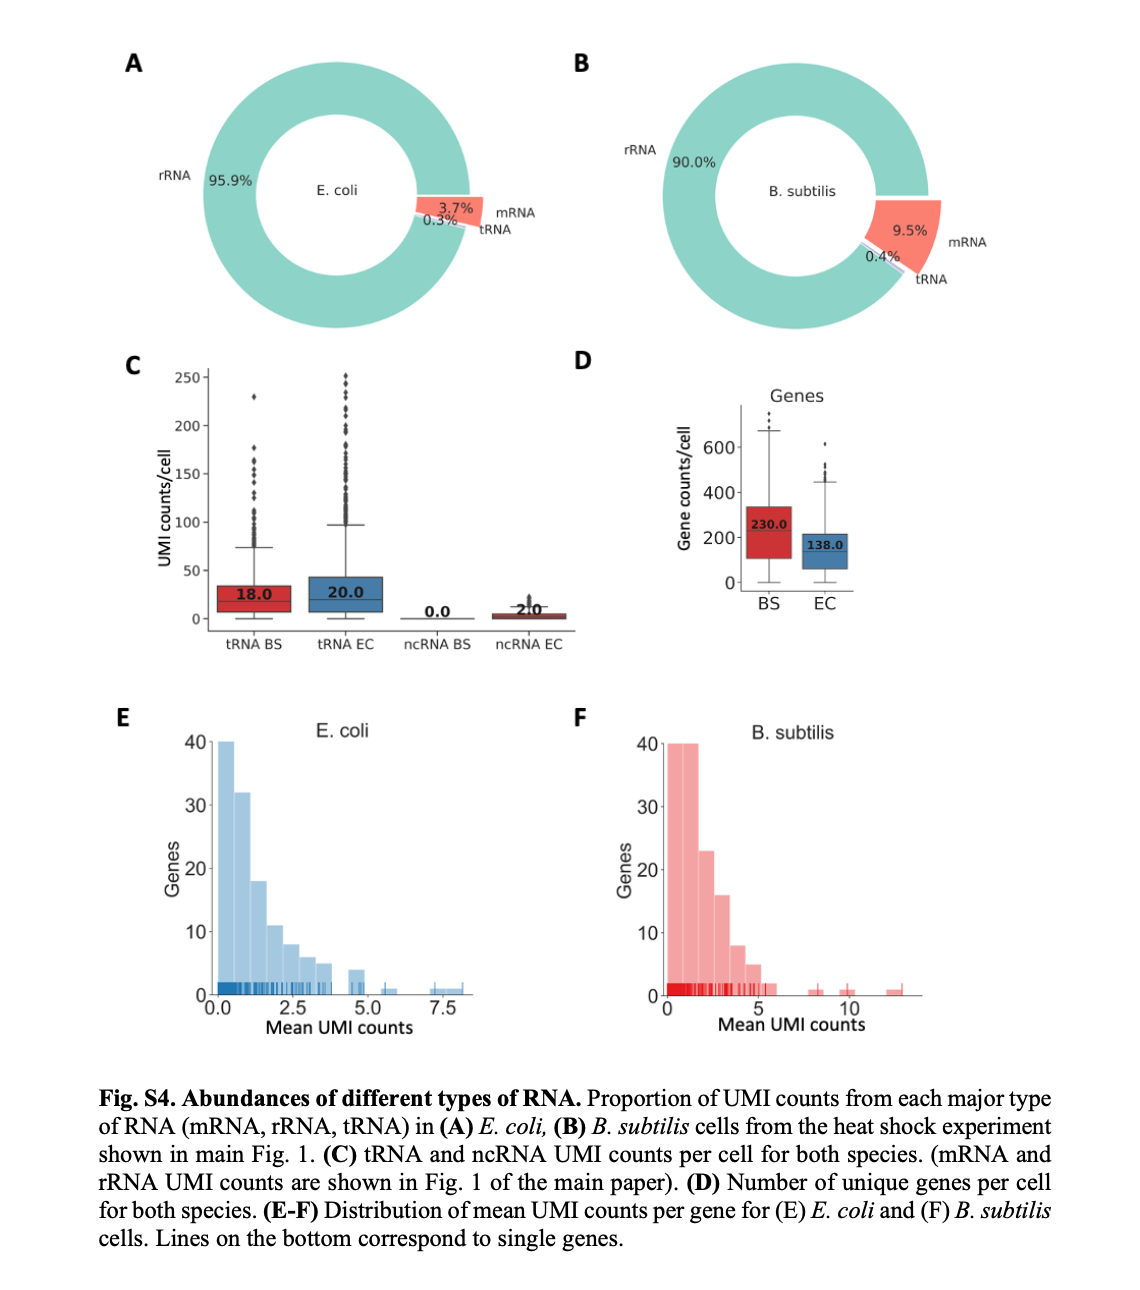
\includegraphics[keepaspectratio]{chapters/../figures/pourcentage_RNA.png}}
\end{itemize}

\bookmarksetup{startatroot}

\chapter{Fitrage des cellules}\label{fitrage-des-cellules}

\begin{itemize}
\item
  reflexion sur le filtrages des cellules est complexe : comme
  mentionnée dans l'article de il existe des methodes de filtrages plus
  ou moins complexes\\
  -filtrage sur le types de reads, globales ou seuils differents entre
  les differentes conditions biologiques -filtrage sur le nombre de
  reads par cellule -filtrage sur le nombre de genes exprimés par
  cellule -filtrage sur le nombre de reads par gene
\item
  filtrage avec un threashold
\item
  dans l'article de kuchina 2021 , ils ont utilisé un seuil de 200 UMI
  par cellule
\item
\item
  preprint de \ldots{} pourrait etre interessant de se focus aussi sur
  rRNA (lien avec growth rate)
\end{itemize}

\bookmarksetup{startatroot}

\chapter{}\label{section}

housekeeping genes

\section{Overview}\label{overview}

This chapter presents the findings of our single-cell RNA-seq analysis
of Pseudomonas, focusing on the division of labor within bacterial
populations.

\section{Single-cell RNA-seq
Analysis}\label{single-cell-rna-seq-analysis}

\subsection{Data Quality and
Preprocessing}\label{data-quality-and-preprocessing}

\subsection{Cell Type Identification}\label{cell-type-identification}

\subsection{Differential Expression
Analysis}\label{differential-expression-analysis}

\subsection{Division of Labor
Patterns}\label{division-of-labor-patterns}

\section{Functional Analysis}\label{functional-analysis}

\subsection{Pathway Enrichment}\label{pathway-enrichment}

\subsection{Gene Set Analysis}\label{gene-set-analysis}

\subsection{Regulatory Network
Analysis}\label{regulatory-network-analysis}

\section{Integration with Previous
Studies}\label{integration-with-previous-studies}

\section{Summary of Key Findings}\label{summary-of-key-findings}

\bookmarksetup{startatroot}

\chapter{Discussion}\label{discussion}

\begin{itemize}
\item
  recepetion tardives des resultats
\item
  mis beaucoup de temps pour le trimming ( 1mois) le temps de comprendre
  la structure de la librairie et
\item
  alternative à Starsolo =\textgreater{}
  BarQC'\textsuperscript{\citeproc{ref-rossello}{11}}
\item
  Nextflow pour le trimming, QC , et STARsolo serait une bonne idée , et
  barQC ; pourrait etre utile pour la communauté
\item
  analyse temporelle , metabolique , bulkRNAseq
\item
  utilisation pour capturer specifique mRNA (voir article : 2 methodes
  existes ; et apres aussi peut etre fait )
\item
  mais je pense deja bioinformatiquement on peut faire des choses pour
  ameliorer reads utilisables
\item
  comparer avec differentes methodes de single cell RNA seq, voir si on
  observe toujours la meme chose ou pas
\item
  versionnement des outils utilisés (renv , singularity, conda)
\item
  rapport fait un template pour rendu propre
\end{itemize}

\section{Interpretation of Key
Findings}\label{interpretation-of-key-findings}

\subsection{Division of Labor
Mechanisms}\label{division-of-labor-mechanisms}

\subsection{Biological Significance}\label{biological-significance}

\subsection{Technical Considerations}\label{technical-considerations}

\section{Comparison with Existing
Literature}\label{comparison-with-existing-literature}

\subsection{Similarities with Previous
Studies}\label{similarities-with-previous-studies}

\subsection{Novel Insights}\label{novel-insights}

\subsection{Discrepancies and Their
Implications}\label{discrepancies-and-their-implications}

\section{Methodological Strengths and
Limitations}\label{methodological-strengths-and-limitations}

\subsection{Technical Advantages}\label{technical-advantages}

\subsection{Potential Limitations}\label{potential-limitations}

\subsection{Future Methodological
Improvements}\label{future-methodological-improvements}

\section{Biological Implications}\label{biological-implications}

\subsection{Ecological Significance}\label{ecological-significance}

\subsection{Evolutionary Perspectives}\label{evolutionary-perspectives}

\subsection{Potential Applications}\label{potential-applications}

\section{Future Research Directions}\label{future-research-directions}

\subsection{Open Questions}\label{open-questions}

\subsection{Suggested Follow-up
Studies}\label{suggested-follow-up-studies}

\subsection{Technical Improvements}\label{technical-improvements}

\section{Conclusion}\label{conclusion}

\bookmarksetup{startatroot}

\chapter{Conclusion and Future Work}\label{conclusion-and-future-work}

\section{Summary of Main Findings}\label{summary-of-main-findings}

\subsection{Key Discoveries}\label{key-discoveries}

\subsection{Methodological
Contributions}\label{methodological-contributions}

\subsection{Biological Insights}\label{biological-insights}

\section{Impact on the Field}\label{impact-on-the-field}

\subsection{Contribution to Single-cell RNA-seq
Methodology}\label{contribution-to-single-cell-rna-seq-methodology}

\subsection{Contribution to Pseudomonas
Research}\label{contribution-to-pseudomonas-research}

\subsection{Broader Implications for Microbial
Ecology}\label{broader-implications-for-microbial-ecology}

\section{Future Research Directions}\label{future-research-directions-1}

\subsection{Technical Improvements}\label{technical-improvements-1}

\subsection{Biological Questions to
Address}\label{biological-questions-to-address}

\subsection{Potential Applications}\label{potential-applications-1}

\section{Final Remarks}\label{final-remarks}

\section{References}\label{references}

\clearpage
% Désactiver l'inclusion des prochaines figures et tableaux dans les listes
\captionsetup[figure]{list=false}
\captionsetup[table]{list=false}

\bookmarksetup{startatroot}

\chapter*{Bibliography}\label{bibliography}
\addcontentsline{toc}{chapter}{Bibliography}

\markboth{Bibliography}{Bibliography}

\phantomsection\label{refs}
\begin{CSLReferences}{0}{0}
\bibitem[\citeproctext]{ref-kuchina2021}
\CSLLeftMargin{1. }%
\CSLRightInline{Kuchina, A. \emph{et al.}
\href{https://doi.org/10.1126/science.aba5257}{Microbial single-cell RNA
sequencing by split-pool barcoding}. \emph{Science} \textbf{371},
eaba5257 (2021).}

\bibitem[\citeproctext]{ref-gaisser2024}
\CSLLeftMargin{2. }%
\CSLRightInline{Gaisser, K. D. \emph{et al.}
\href{https://doi.org/10.1038/s41596-024-01007-w}{High-throughput
single-cell transcriptomics of bacteria using combinatorial barcoding}.
\emph{Nature Protocols} \textbf{19}, 3048--3084 (2024).}

\bibitem[\citeproctext]{ref-morris2012}
\CSLLeftMargin{3. }%
\CSLRightInline{Morris, J. J., Lenski, R. E. \& Zinser, E. R.
\href{https://doi.org/10.1128/mBio.00036-12}{The black queen hypothesis:
Evolution of dependencies through adaptive gene loss}. \emph{mBio}
\textbf{3}, e00036--12 (2012).}

\bibitem[\citeproctext]{ref-morris2014}
\CSLLeftMargin{4. }%
\CSLRightInline{Morris, E. K. \emph{et al.}
\href{https://doi.org/10.1002/ece3.1155}{Choosing and using diversity
indices: insights for ecological applications from the German
Biodiversity Exploratories}. \emph{Ecology and Evolution} \textbf{4},
3514--3524 (2014).}

\bibitem[\citeproctext]{ref-estrela2016}
\CSLLeftMargin{5. }%
\CSLRightInline{Estrela, S., Kerr, B. \& Morris, J. J.
\href{https://doi.org/10.1016/j.mib.2016.04.007}{Transitions in
individuality through symbiosis}. \emph{Current Opinion in Microbiology}
\textbf{31}, 191--198 (2016).}

\bibitem[\citeproctext]{ref-nishimura2025}
\CSLLeftMargin{6. }%
\CSLRightInline{Nishimura, M., Takahashi, K. \& Hosokawa, M. Recent
advances in single-cell RNA sequencing of bacteria: Techniques,
challenges, and applications. \emph{Journal of Bioscience and
Bioengineering} (2025)
doi:\href{https://doi.org/10.1016/j.jbiosc.2025.01.008}{10.1016/j.jbiosc.2025.01.008}.}

\bibitem[\citeproctext]{ref-ostner}
\CSLLeftMargin{7. }%
\CSLRightInline{Ostner, J. \emph{et al.} BacSC: A general workflow for
bacterial single-cell RNA sequencing data analysis.
doi:\href{https://doi.org/10.1101/2024.06.22.600071}{10.1101/2024.06.22.600071}.}

\bibitem[\citeproctext]{ref-brettner2024}
\CSLLeftMargin{8. }%
\CSLRightInline{Brettner, L. \& Geiler-Samerotte, K. Single-cell
heterogeneity in ribosome content and the consequences for the growth
laws. \emph{bioRxiv: The Preprint Server for Biology} 2024.04.19.590370
(2024)
doi:\href{https://doi.org/10.1101/2024.04.19.590370}{10.1101/2024.04.19.590370}.}

\bibitem[\citeproctext]{ref-chen2018}
\CSLLeftMargin{9. }%
\CSLRightInline{Chen, S., Zhou, Y., Chen, Y. \& Gu, J.
\href{https://doi.org/10.1093/bioinformatics/bty560}{Fastp: An
ultra-fast all-in-one FASTQ preprocessor}. \emph{Bioinformatics}
\textbf{34}, i884--i890 (2018).}

\bibitem[\citeproctext]{ref-martin2011}
\CSLLeftMargin{10. }%
\CSLRightInline{Martin, M.
\href{https://doi.org/10.14806/ej.17.1.200}{Cutadapt removes adapter
sequences from high-throughput sequencing reads}. \emph{EMBnet.journal}
\textbf{17}, 10--12 (2011).}

\bibitem[\citeproctext]{ref-rossello}
\CSLLeftMargin{11. }%
\CSLRightInline{Rossello, M., Tandonnet, S. \& Almudi, I. BarQC: Quality
Control and Preprocessing for SPLiT-Seq Data.
doi:\href{https://doi.org/10.1101/2025.02.04.635005}{10.1101/2025.02.04.635005}.}

\end{CSLReferences}

\cleardoublepage
\phantomsection
\addcontentsline{toc}{part}{Appendices}
\appendix

\chapter{}\label{section-1}

\begin{itemize}
\tightlist
\item
  plan de plaque
\item
  librairies avec TSO
\item
  tableau choix de profondeur / nombre de cellules
\end{itemize}

\chapter{Annexe B: erferfrefref}\label{annexe-b}

\chapter{Annexe C: codcefe}\label{annexe-c}

\clearpage
\thispagestyle{empty}
\vspace*{\fill}
\vspace*{\fill}
\clearpage



% Back cover content
\newpage  % Force a new page
\thispagestyle{empty}  % Page without header or footer
\begin{center}
  {\Huge \textbf{Master's Thesis in Bioinformatics}} \\[2cm]
  {\Large \textbf{University of Rennes}} \\[1cm]
  
\includegraphics[width=0.4\textwidth]{figures/logo_Univ_Rennes.png} \\[1cm]
  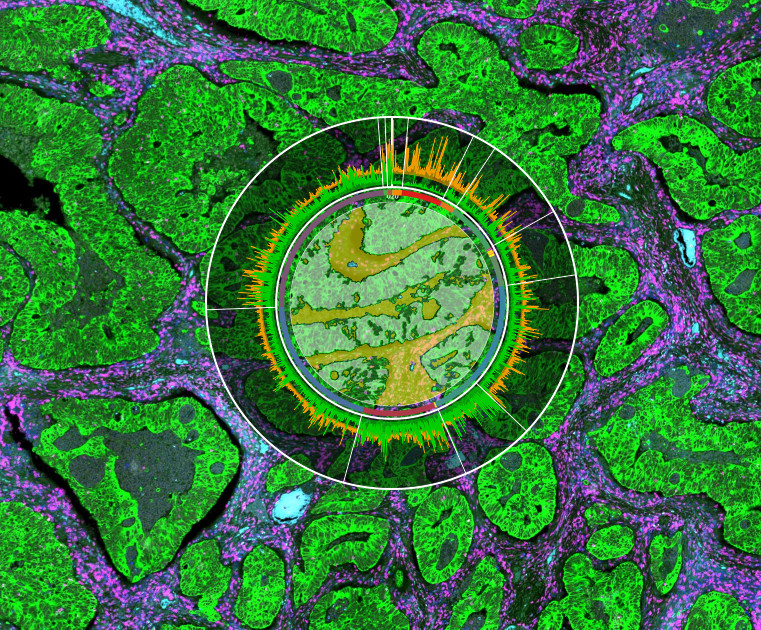
\includegraphics[width=0.6\textwidth]{figures/couverture.jpg} \\[1cm]
  \begin{minipage}{0.8\textwidth}
    \centering
    \textit{This thesis was conducted in the framework of the Master's program in Bioinformatics at the University of Rennes. The research presented here contributes to the field of computational biology and bioinformatics.}
  \end{minipage} \\[1cm]
  \begin{minipage}{0.8\textwidth}
    \centering
    \small
    \textit{© Valentin Goupille - ?meta:year \\ All rights reserved}
  \end{minipage}
\end{center} 


\end{document}
